\documentclass{article}

\usepackage[utf8]{inputenc}
\usepackage[T1]{fontenc}
\usepackage[serbian]{babel}
\usepackage{amsmath}
\usepackage{amssymb}
\usepackage{graphicx}
\usepackage{hyperref}
\usepackage{geometry}
\usepackage{booktabs}
\usepackage{array}
\usepackage{float}
\usepackage{xcolor}
\usepackage{titling}
\usepackage{subcaption}
% Diskretne boje
\definecolor{linkblue}{RGB}{30, 90, 140}
\definecolor{titlegray}{RGB}{55, 55, 55}
\definecolor{lightgray}{RGB}{120, 120, 120}

% Hyperlink / citation colors
\hypersetup{
    colorlinks=true,
    linkcolor=linkblue,
    citecolor=linkblue,
    urlcolor=linkblue
}

\geometry{a4paper, margin=1in}

\begin{document}

\begin{titlepage}
    \centering

    \vspace*{1.5cm}

    {\large\color{titlegray}
    UNIVERZITET U BEOGRADU\\[0.15cm]
    ELEKTROTEHNIČKI FAKULTET
    }

    \vspace{2.8cm}

    {\color{linkblue}\rule{0.85\textwidth}{1.2pt}}

    \vspace{0.7cm}

    {\Huge\bfseries\color{titlegray}
    Interaktivno generisanje ljudskog pokreta u virtuelnoj realnosti
    \par}

    \vspace{0.3cm}

    {\LARGE\color{linkblue}
    Zadavanje ograničenja demonstracijom i difuzioni modeli pokreta
    \par}

    \vspace{0.7cm}

    {\color{linkblue}\rule{0.85\textwidth}{1.2pt}}

    \vspace{1.2cm}

    {\large
    Projekat iz predmeta
    \par}

    \vfill

    \begin{tabular}{@{}ll@{}}
        \textcolor{lightgray}{Student:} &
        \textbf{Anastasija Rakić} \\[0.25cm]

        % TODO: potvrditi tačan naziv predmeta
        \textcolor{lightgray}{Predmet:} &
        Virtuelna realnost \\[0.25cm]

        \textcolor{lightgray}{Akademska godina:} &
        2026/27
    \end{tabular}

    \vspace{1.8cm}

    {\color{lightgray}
    Beograd, 2026.
    }

    \vspace{0.7cm}

\end{titlepage}

\begin{abstract}

Difuzioni modeli ljudskog pokreta omogućavaju generisanje raznovrsnih i uverljivih pokreta iz tekstualnog opisa, ali njihova praktična vrednost u interaktivnim i robotičkim primenama zavisi od toga koliko prirodno korisnik može da zada prostorna i vremenska ograničenja koja generisani pokret mora da ispuni. Ovaj rad predstavlja sistem u kome se ograničenja zadaju \emph{demonstracijom}: korisnik u virtuelnoj realnosti (ili u ekvivalentnom simuliranom režimu na ekranu) pokazuje putanju kretanja, tačke dodira na površinama i ključne poze tela, a sistem od tih demonstracija sastavlja skup kinematičkih ograničenja za difuzioni model pokreta Kimodo. Generisani pokret se zatim reprodukuje u istoj sceni, na skinovanom humanoidnom karakteru, među nameštajem i robotskim manipulatorima sa kojima virtuelni čovek treba da deli prostor.

Sistem je realizovan kao klijent--server arhitektura: Unity klijent (OpenXR za VR, sa punom podrškom za rad bez opreme) zadužen je za scenu, interakciju i reprodukciju, dok serverska strana (FastAPI, PyTorch) izvršava generisanje i naknadnu obradu pokreta. Pošto model pokreta nema svest o sceni, klijent planira putanje prilaska koje zaobilaze prepreke i prevodi ih u ograničenja putanje korena tela. Rad opisuje ideju sistema, korišćene modele i tehnologije, ključne detalje implementacije, jedan reprezentativan scenario upotrebe, kao i ostvarene rezultate i ograničenja.

\end{abstract}

\section{Uvod}
\label{sec:introduction}

Generisanje ljudskog pokreta iz tekstualnog opisa postalo je, zahvaljujući razvoju dubokih generativnih modela, dovoljno kvalitetno da se može koristiti ne samo za animaciju već i kao komponenta interaktivnih i robotičkih sistema. Modeli poput MDM-a \cite{tevet2022humanmotiondiffusionmodel} i novijeg modela Kimodo \cite{rempe2026kimodo} mogu iz kratkog tekstualnog opisa da generišu čitave sekvence ljudskog pokreta koje odgovaraju zadatoj radnji i zadržavaju prirodnu varijabilnost ljudskog kretanja.

Sam tekstualni opis, međutim, uglavnom određuje \emph{šta} osoba treba da uradi, ali ne i dovoljno precizno \emph{gde} i \emph{kako} radnja treba da bude izvedena u konkretnoj sceni. Na primer, opis ,,osoba priđe stolu i pređe rukom po njegovoj površini`` ne određuje kom stolu treba prići, sa koje strane, kojom putanjom kroz prostoriju, gde osoba treba da stane niti gde tačno šaka treba da dodirne površinu. U generičkim skupovima podataka takva prostorna neodređenost nije problem, ali postaje značajna kada generisani čovek treba da postoji u konkretnoj virtuelnoj sceni zajedno sa nameštajem, radnim površinama i robotima.

Jedan način rešavanja ovog problema jeste eksplicitno numeričko zadavanje svih potrebnih koordinata i vremenskih trenutaka. Takav interfejs, međutim, nije naročito prirodan korisniku. Prostorni deo zadatka često je mnogo jednostavnije pokazati nego opisati ili numerički definisati. Korisnik može da prođe željenom putanjom, pokaže mesto dodira na površini ili zauzme željenu pozu, a sistem zatim može da tu demonstraciju pretvori u odgovarajuća ograničenja generativnog modela.

Virtuelna stvarnost predstavlja prirodan interfejs za ovakav način zadavanja pokreta. Korisnik se već nalazi u istoj geometrijskoj sceni u kojoj će se generisani pokret izvršavati. Kretanje korisnika kroz prostor može se direktno interpretirati kao željena putanja tela, kretanje kontrolera po površini kao trag dodira šake, a trenutni položaj vizira i kontrolera kao delimična demonstracija poze.

Cilj ovog projekta je zato razvoj interaktivnog sistema koji kombinuje tekstualno generisanje pokreta i prostorna ograničenja zadata demonstracijom. Tekst određuje semantiku ponašanja, dok demonstracija određuje njegovu prostornu realizaciju. Generativni model pri tome ne kopira direktno kretanje korisnika, kao kod klasične teleoperacije ili motion-capture reprodukcije, već generiše novi pokret koji zadovoljava demonstrirana ograničenja.

Poseban motivacioni kontekst predstavljaju sistemi saradnje čoveka i robota. U takvim sistemima često je potrebno generisati više mogućih ljudskih ponašanja u zajedničkom radnom prostoru kako bi se ispitala bezbednost, ergonomija ili reakcija robota na različite ljudske akcije. U razvijenoj sceni zato se pored virtuelnog čoveka nalaze i robotski manipulatori Franka Emika Panda. Demonstracije obuhvataju ponašanja poput prilaska radnoj površini, posezanja, dodira i zauzimanja određene pozicije u blizini robota.

Doprinos projekta obuhvata:
\begin{itemize}
    \item interaktivni VR i desktop klijent u okruženju Unity za zadavanje putanja kretanja, tragova dodira i ključnih poza;
    \item prevođenje demonstracija korisnika u kinematička ograničenja koja prihvata model Kimodo;
    \item konstrukciju ograničenja poze na osnovu svega tri direktno praćene tačke tela, odnosno vizira i dva kontrolera;
    \item planiranje putanje korena tela kroz poznatu virtuelnu scenu radi izbegavanja prepreka koje sam generativni model ne opaža;
    \item generisanje pokreta na serverskoj strani i njegov prenos između različitih koordinatnih sistema;
    \item retargetovanje generisanog pokreta na skinovani humanoidni karakter i dodatnu korekciju kontakta na ciljnom skeletu;
    \item interaktivnu režiju već generisanih likova: promenu ponašanja, nadovezivanje sledeće radnje, isecanje dela klipa i ručno pozicioniranje, i na ekranu i u VR režimu;
    \item prostorna ograđivanja pri reprodukciji, kojima se garantuje da generisani lik ne napušta prostoriju i ne prolazi telom kroz nameštaj;
    \item čuvanje kompletne demonstracije u JSON formatu, tako da ista specifikacija kasnije može biti korišćena i izvan Unity okruženja.
\end{itemize}

Ostatak rada organizovan je na sledeći način. Poglavlje~\ref{sec:models} opisuje korišćeni generativni model i softverske komponente sistema. Poglavlje~\ref{sec:implementation} opisuje arhitekturu, način zadavanja ograničenja, planiranje putanje, konstrukciju poza, retargetovanje i interaktivnu režiju generisanih likova. Poglavlje~\ref{sec:scenario} prikazuje kompletan scenario korišćenja, dok poglavlja~\ref{sec:results} i~\ref{sec:limitations} analiziraju ostvarene rezultate, trenutna ograničenja sistema i moguće pravce njegovog daljeg razvoja.

% ============================================================
% 2. MODELI I TEHNOLOGIJE
% ============================================================

\section{Korišćeni modeli i tehnologije}
\label{sec:models}

\subsection{Kimodo: difuzioni model pokreta sa ograničenjima}

Kimodo \cite{rempe2026kimodo} je generativni model ljudskog pokreta zasnovan na difuzionom procesu i Transformer arhitekturi. Njegov izlaz nije pojedinačna poza već vremenska sekvenca konfiguracija ljudskog skeleta. Model je uslovljen tekstualnim opisom pokreta, ali za ovaj projekat je posebno značajno to što podržava i eksplicitna kinematička ograničenja nad generisanom sekvencom.

U standardnom difuzionom procesu početni uzorak predstavlja šum, koji se kroz niz iteracija postepeno transformiše u strukturiranu sekvencu pokreta \cite{ho2020denoisingdiffusionprobabilisticmodels}. Tekstualni i kinematički uslovi utiču na ovaj proces tako da konačni pokret istovremeno odgovara zadatoj radnji i prolazi kroz tražene prostorne konfiguracije. Za vođenje generisanja koristi se pristup bez posebnog klasifikatora \cite{ho2022classifierfreediffusionguidance}.

Kimodo podržava više vrsta ograničenja koje se mogu kombinovati u okviru iste sekvence:
\begin{itemize}
    \item \textbf{putanja korena} (\textit{root2d}), koja određuje položaj tela u ravni tla kroz vreme;
    \item \textbf{ograničenja pojedinačnih efektora}, kao što su leva ili desna šaka i stopala;
    \item \textbf{ograničenja kompletne poze} (\textit{fullbody}) u izabranim vremenskim trenucima;
    \item \textbf{tekstualni opis ponašanja}, koji može sadržati jednu radnju ili više uzastopnih semantičkih segmenata.
\end{itemize}

Važna osobina ovakve reprezentacije jeste da ograničenja ne moraju definisati svaku koordinatu svakog zgloba. Na primer, položaj desne šake može biti fiksiran u određenom trenutku, dok položaj lakta, torza i nogu ostaje slobodan. Model tada bira konfiguraciju koja zadovoljava eksplicitno ograničenje, ali istovremeno ostaje u skladu sa distribucijom prirodnog ljudskog pokreta naučenom tokom obuke. Upravo ova osobina omogućava da demonstracija korisnika bude relativno retka i nepotpuna.

Model radi u kanonskom koordinatnom sistemu. Putanja korena se pre generisanja translira tako da njen početak odgovara koordinatnom početku modela, a nakon generisanja rezultat se transformiše nazad u koordinatni sistem virtuelne scene.

Pored samog difuzionog uzorkovanja koristi se i naknadna obrada pokreta. Ona uključuje korekciju klizanja stopala i postupak \textit{constraint snapping}, kojim se odabrani kadrovi dodatno dovode na tačno zadate vrednosti. Ovo je posebno značajno za kontakte, jer mala greška koja vizuelno nije značajna tokom slobodnog pokreta može postati očigledna kada šaka treba precizno da dodirne površinu stola.

Tekstualni opis kodira se enkoderom LLM2Vec \cite{llm2vec2024} zasnovanim na modelu Llama-3-8B. Zbog veličine enkodera, približno $16\,GB$, njegova upotreba predstavlja značajan deo vremena obrade novog opisa. Zbog toga je kodiranje implementirano lenjo i sa keširanjem. Tekstualni opis se kodira samo pri prvom korišćenju, dok se pri svim narednim generisanjima odgovarajući vektor učitava iz keša.

Važno ograničenje modela jeste odsustvo eksplicitne reprezentacije okruženja. Kimodo ne dobija geometriju prostorije, prepreka, stolova niti robota. Za njega postoji samo telo i skup zadatih ograničenja. Zbog toga se deo problema koji zavisi od scene rešava na strani Unity klijenta, a rezultat se modelu prosleđuje u obliku dodatnih kinematičkih ograničenja.

\subsection{Unity klijent}

Klijentska strana je realizovana u okruženju Unity (URP), sa podrškom za OpenXR uređaje. Ista aplikacija radi i bez VR opreme: svim interakcijama se može upravljati mišem i tastaturom, uključujući poseban \emph{simulirani rig} u kome kamera preuzima ulogu vizira, a dve virtuelne šake se pozicioniraju mišem --- što omogućava razvoj i testiranje celog toka bez opreme. Za reprodukciju generisanog pokreta na skinovanom humanoidnom karakteru koristi se Unity Mecanim sistem (\textit{HumanPoseHandler}), koji pokret prenosi u prostoru mišićnih koordinata i time ga retargetuje na telo drugačijih proporcija. Robotski manipulatori Franka Emika Panda uvezeni su iz URDF opisa pomoću zvaničnog Unity URDF uvoznika.

\subsection{Serverska strana}

Generisanje se izvršava na lokalnom serveru (FastAPI, PyTorch) pokrenutom u WSL2 okruženju, na grafičkoj kartici NVIDIA RTX 5070 Ti (12\,GB). Klijent i server komuniciraju JSON zahtevima preko HTTP-a: zahtev sadrži tekstualni opis, trajanje, putanju korena, tragove dodira, položaje tela i ključne poze, a odgovor sadrži generisani pokret (lokalne rotacije zglobova i putanju korena) u obliku pogodnom za reprodukciju u Unity-ju. Svaka generacija se arhivira (zahtev, izgrađena ograničenja, pokret), što omogućava naknadnu analizu i reprodukciju.

% ============================================================
% 3. IMPLEMENTACIJA
% ============================================================

\section{Implementacija}
\label{sec:implementation}

\subsection{Arhitektura i tok podataka}

Sistem je organizovan kao klijent--server arhitektura sa jasnim razdvajanjem interakcije sa scenom i računarski zahtevnog generisanja pokreta. Unity klijent poseduje kompletnu geometriju virtuelnog okruženja i podatke o korisničkoj interakciji, dok serverska strana poseduje generativni model i procedure za obradu njegovog izlaza.

Kompletan tok prikazan je na slici~\ref{fig:system_pipeline}. Korisnik najpre zadaje tekstualni opis ponašanja i jednu ili više prostornih demonstracija. Unity registruje pozicije vizira i kontrolera, tačke na površinama i vremenske trenutke demonstracije. Sirovi podaci zatim se obrađuju i pretvaraju u semantička ograničenja koja odgovaraju rečniku modela Kimodo.

\begin{figure}[H]
    \centering
    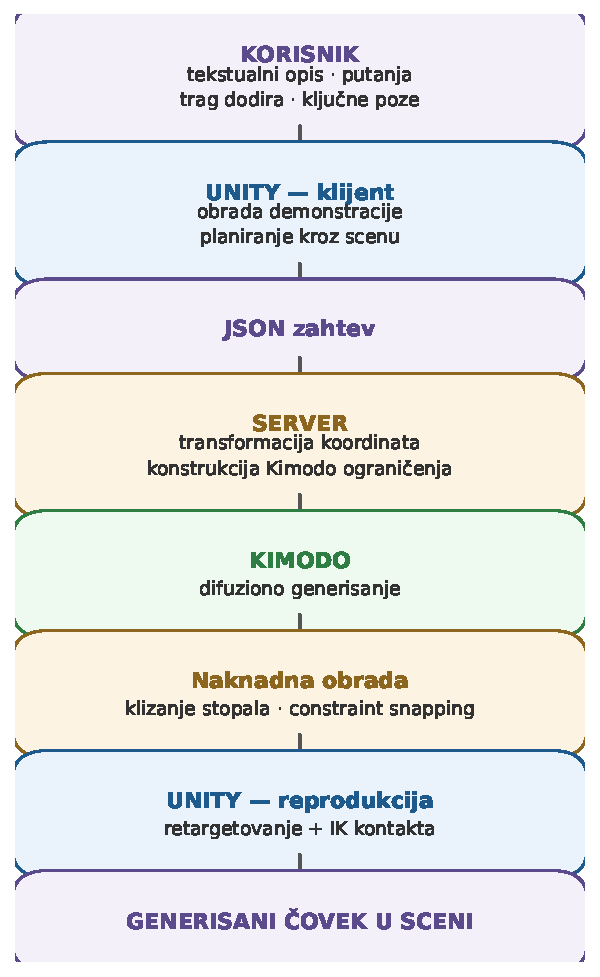
\includegraphics[width=0.52\textwidth]{figures/pipeline.pdf}
    \caption{Kompletan tok sistema od demonstracije korisnika do reprodukcije
    generisanog pokreta. Unity obrađuje informacije koje zavise od scene,
    dok server transformiše ograničenja i izvršava generisanje modelom Kimodo.}
    \label{fig:system_pipeline}
\end{figure}

Ukoliko je zadat cilj u sceni, klijent dodatno koristi geometriju prepreka da izračuna putanju prilaska. Tako dobijeni podaci, zajedno sa tekstualnim opisom, trajanjem pokreta i vremenskim oznakama, serijalizuju se u JSON zahtev i šalju serveru.

Server proverava zahtev, transformiše ograničenja u koordinatni sistem modela i obavlja njihovu kanonizaciju. Nakon toga Kimodo generiše pokret, nad kojim se izvršavaju korekcija klizanja stopala i privlačenje na eksplicitno zadate ciljeve. Rezultat se zatim transformiše nazad u koordinatni sistem Unity-ja i šalje klijentu.

Na strani klijenta generisane rotacije i globalno kretanje prenose se na ciljni humanoidni karakter. Poslednji korak predstavlja lokalna korekcija kontakta pomoću inverzne kinematike, nakon čega se završeni pokret reprodukuje u originalnoj virtuelnoj sceni.

Poseban praktični problem predstavlja činjenica da Unity koristi levoruki, a Kimodo desnoruki koordinatni sistem. Na granici sistema zato se vrši eksplicitna transformacija položaja i orijentacija. Za položaje se menja znak odgovarajuće ose, dok se za kvaternione primenjuje odgovarajuće preslikavanje komponenti. Transformacija je proverena i semantički, zadavanjem ograničenja samo nad levom odnosno samo nad desnom šakom, čime je potvrđeno očuvanje hiralnosti.

\subsection{Zadavanje ograničenja demonstracijom}
\label{sec:interactions}

Osnovna ideja interfejsa jeste da korisnik ne mora direktno da poznaje reprezentaciju ograničenja koju očekuje generativni model. Umesto numeričkog zadavanja koordinata i vremena, korisnik izvodi jednostavne prostorne demonstracije, a sistem ih automatski prevodi u odgovarajuće strukture.

Sve demonstracije nalaze se na zajedničkoj vremenskoj osi, što omogućava njihovo kombinovanje. Na primer, korisnik može prvo demonstrirati putanju prilaska, zatim zadati mesto kontakta desne šake i konačno zauzeti ključnu pozu koju lik treba da postigne nakon dolaska.

U VR režimu implementirane su tri osnovne vrste demonstracije.

\begin{itemize}
    \item \textbf{Trag dodira.} Dok korisnik drži desni okidač, putanja kontrolera se uzorkuje kroz vreme. Za svaki uzorak određuje se najbliža odgovarajuća površina, a položaj se projektuje na nju. Dobijeni niz tačaka postaje vremenski niz ograničenja desne šake. Na taj način korisnik može, na primer, jednim prirodnim pokretom da pokaže duž koje linije šaka treba da pređe preko stola.

    \item \textbf{Putanja kretanja.} Dok korisnik drži levi okidač, položaj vizira projektovan na ravan tla periodično se uzorkuje. Dobijene tačke formiraju \textit{root2d} ograničenje koje opisuje gde koren tela treba da se nalazi tokom kretanja.

    \item \textbf{Ključna poza.} Pritiskom na dugme X registruju se položaji obe šake, položaj korisnika, visina vizira i njegov horizontalni pravac gledanja. Ovi podaci predstavljaju parcijalno posmatranje ljudske konfiguracije koje se naknadno pretvara u ograničenje za generativni model. Odmah po snimanju poza se prikazuje kao poluprovidna štap-figura na mestu demonstracije, tako da korisnik i pre generisanja vidi tačno šta je zabeleženo.
\end{itemize}

Pošto svako zadato ograničenje mora biti i \emph{izvodljivo}, sistem pri snimanju poze primenjuje nekoliko provera. Položaji šaka se ograničavaju na sferu dohvata ruke oko grudi sintetisanog tela; ukoliko korisnik zada dalju tačku, ona se privlači na granicu dohvata, uz vidljivu napomenu. Vremenski razmak između uzastopnih poza automatski se produžava ako je kraći od vremena potrebnog da se pređe rastojanje između njih hodom, čime se sprečava fizički nemoguće ,,teleportovanje``. Konačno, kao informacija o visini tela koriste se samo verodostojne visine vizira (između $1.2$ i $2.1\,m$); van tog opsega, na primer kada u simuliranom režimu kamera stoji nisko, pretpostavlja se uspravan stav. Bez ovih provera protivrečna ograničenja mogu destabilizovati difuziono uzorkovanje i proizvesti degenerisan pokret, što je tokom razvoja i empirijski primećeno.

Preslikavanje pojedinačnih demonstracija u reprezentaciju modela sažeto je prikazano na slici~\ref{fig:demo_mapping}.

\begin{figure}[H]
    \centering
    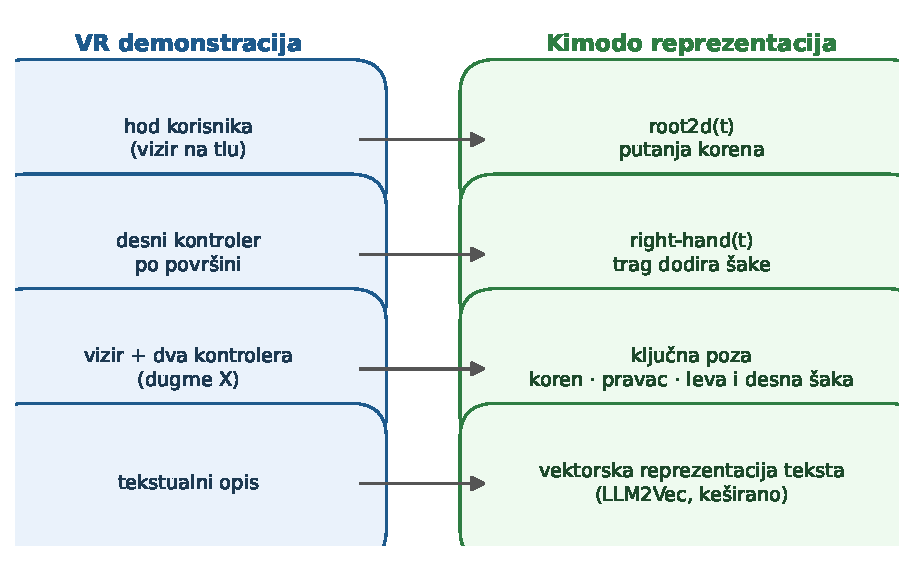
\includegraphics[width=0.85\textwidth]{figures/demo_mapping.pdf}
    \caption{Prevođenje VR demonstracija u rečnik ograničenja modela Kimodo.
    Svaka vrsta demonstracije preslikava se u odgovarajuću vrstu ograničenja,
    uz očuvanje vremenskih oznaka zajedničke vremenske ose.}
    \label{fig:demo_mapping}
\end{figure}

U svim slučajevima čuva se i vremenska informacija. Ovo je važno zato što ista prostorna tačka ima potpuno različito značenje ukoliko treba da bude dostignuta na početku, u sredini ili na kraju pokreta. Vremenske oznake demonstracije zato se normalizuju u odnosu na trajanje generisanog klipa.

Kratke demonstracije kontakta dodatno se vremenski proširuju. Cilj nije da se proizvoljno promeni korisnikova demonstracija, već da se generativnom modelu pruži dovoljno jak vremenski signal. Jedna izolovana tačka ili veoma kratak trag mogu imati mali uticaj tokom difuzionog uzorkovanja, dok kratki prozor susednih ograničenja znatno stabilnije određuje željeni kontakt.

Isti princip interakcije dostupan je i bez VR opreme. U desktop režimu klik na površinu definiše cilj kontakta, desni klik dodaje tačke putanje, dok poseban simulirani rig omogućava nezavisno pozicioniranje leve i desne šake. Na taj način kompletan pipeline može da se razvija i testira bez povezanog VR uređaja.

Interaktivne površine scene su eksplicitno registrovane: autor scene u listu površina prevlači radne ploče, police ili čitave komade nameštaja, a pored vidljivih objekata podržane su i \emph{nevidljive zone} --- prazni objekti sa graničnim kolajderom kojima se interaktivnim proglašava tačno određeni deo nameštaja, na primer jedna polica u ormaru ili prednja polovina stola. Klik pri zadavanju dodira bira najbližu \emph{registrovanu} površinu duž zraka, pa telo ormara ne blokira zonu u njegovoj unutrašnjosti. Pri pokretanju sistem za svaku registrovanu površinu iscrtava okvir na njenoj gornjoj plohi i proverava verodostojnost njene visine u odnosu na visinu generisanog čoveka (uvek $1.75\,m$), čime se greške u razmeri nameštaja otkrivaju pre prvog generisanja.

Cela demonstracija može se serijalizovati u JSON datoteku. Datoteka sadrži tekstualni opis, trajanje, prostorne ciljeve i vremenske oznake, pa se ista demonstracija može ponovo generisati bez ponavljanja korisničke interakcije.

\subsection{Planiranje prilaza sa zaobilaženjem prepreka}
\label{sec:planning}

Jedna od centralnih razlika između generisanja pokreta iz teksta i generisanja pokreta u konkretnoj VR sceni jeste potreba za geometrijskom konzistentnošću sa okruženjem. Kimodo ne prima geometriju scene kao ulaz i zato ne može sam da zaključi da se između početne pozicije čoveka i ciljnog stola nalazi prepreka.

Ovaj problem se rešava pre generisanja, na strani Unity klijenta. Za svaku relevantnu prepreku formira se dvodimenzionalni pravougaoni otisak u ravni poda. Otisak se zatim proširuje za efektivni radijus ljudskog tela i dodatnu sigurnosnu marginu. U trenutnoj implementaciji ukupna margina iznosi $0.36\,m$.

Najpre se proverava da li direktan segment između početnog položaja i cilja preseca neku od proširenih prepreka. Za test preseka koristi se Liang--Barsky algoritam. Ukoliko je direktna putanja slobodna, ona se koristi bez dodatnih tačaka.

Ako postoji prepreka, generišu se kandidati koji prolaze preko jednog ili dva njena ugla. Za svaki kandidat proverava se kolizija svih segmenata, a među validnim kandidatima bira se onaj sa najmanjom ukupnom dužinom. Time se dobija jednostavan planer dovoljan za relativno strukturisanu laboratorijsku scenu.

Geometrijska putanja zatim se vremenski parametrizuje pretpostavljenom brzinom hoda od $1.3\,m/s$. Tako dobijeni parovi položaja i vremena pretvaraju se u \textit{root2d} ograničenje modela.

Dodatni problem pojavljuje se nakon dolaska na cilj. Difuzioni model ne interpretira poslednju tačku putanje kao trajnu zabranu daljeg kretanja. Ako tekst i dalje semantički odgovara hodanju, model može nakon dolaska nastaviti da pomera koren tela. Zbog toga se nakon dolaska dodaju ponovljena ograničenja istog položaja u kasnijim vremenskim trenucima. Na ovaj način cilj se ne definiše samo kao tačka kroz koju treba proći, već kao mesto na kome telo treba da ostane tokom izvođenja sledećeg dela zadatka.

Sa ciljem su povezana još dva geometrijska detalja. Prvo, mesto stajanja ispred zadate tačke dodira ne sme se naći \emph{unutar} otiska nameštaja: kod dubokih komada, poput ormara ili komode, naivno postavljanje na fiksno rastojanje od tačke dodira završava u unutrašnjosti otiska, a planer tada ne može da pronađe validnu putanju do cilja. Mesto stajanja se zato iterativno izgurava iz proširenog otiska dodirnutog komada, u smeru ka posmatraču, i prikazuje se posebnim markerom pre generisanja. Drugo, visina kukova u sintetisanoj pozi za ograničenje dodira prilagođava se \emph{visini ciljne tačke}: za ciljeve iznad približno $0.65\,m$ telo ostaje uspravno, dok se za niže ciljeve (donje fioke, predmeti blizu poda) visina kukova srazmerno spušta. Ovo je suštinsko za niske dodire, jer bi fiksirana stojeća visina korena istovremeno činila cilj nedostižnim za ruku i eksplicitno \emph{zabranjivala} modelu da čučne.

\subsection{Ograničenja poza iz tri praćene tačke}
\label{sec:poses}

Standardni VR sistem ne meri kompletnu konfiguraciju ljudskog tela. U korišćenoj postavci direktno su dostupne samo tri praćene tačke: vizir i dva ručna kontrolera. Nasuprot tome, generativni model operiše nad kompletnim skeletom. Zbog toga je potreban međukorak kojim se parcijalna demonstracija korisnika pretvara u reprezentaciju pogodnu za model.

Za svaku zabeleženu ključnu pozu najpre se instancira neutralna konfiguracija referentnog skeleta. Njena horizontalna orijentacija postavlja se prema pravcu gledanja korisnika, dok se položaj korena određuje iz projektovanog položaja vizira u ravni poda.

Visina korisnika predstavlja dodatnu informaciju. Promena visine vizira u odnosu na referentnu uspravnu konfiguraciju koristi se za procenu vertikalnog pomeranja korena. Time jednostavne promene visine tela, kao što su čučanj ili spuštanje, mogu da ostanu prisutne u rezultujućoj konfiguraciji.

Položaji ruku rešavaju se zasebno. Za svaku ruku poznati su položaj ramena u trenutno sintetisanoj konfiguraciji i željeni položaj šake dobijen iz VR kontrolera. Položaj lakta izračunava se dvokosnom inverznom kinematikom za lanac rame--lakat--šaka. Dužine segmenata uzimaju se iz referentnog skeleta, a ugao lakta dobija se primenom zakona kosinusa.

Važno je da sintetisana poza ne predstavlja pokušaj rekonstrukcije stvarnog tela korisnika. Njena uloga je samo da iz retkih VR merenja proizvede konzistentan skelet iz kojeg se mogu izdvojiti ograničenja koja prihvata Kimodo.

U model se zato ne fiksira čitava rekonstruisana poza. Eksplicitno se ograničavaju položaji leve i desne šake, položaj korena i dominantni pravac tela, dok položaji laktova, konfiguracija nogu i orijentacije šaka ostaju slobodni. Generativni model na taj način može sam da izabere prirodnu realizaciju poze koja ispunjava demonstrirane prostorne ciljeve.

Tokom razvoja identifikovana su dva detalja koja značajno utiču na tačnost. Prvi je način imenovanja ograničenja. Naknadna obrada modela razlikuje semantičke grupe kao što su \textit{left-hand} i \textit{right-hand}. Ukoliko se obe ruke proslede kroz generički imenovanu grupu, deo naknadne obrade može da je preskoči. Zbog toga se ograničenja dve ruke formiraju kao zasebni skupovi.

Drugi problem odnosi se na vremensku gustinu ograničenja. Jedan izolovan ključni kadar predstavlja relativno slab signal tokom difuzionog uzorkovanja. Zbog toga se svaka demonstrirana poza predstavlja kratkim vremenskim prozorom od približno $\pm0.13\,s$, pri čemu se ograničenje primenjuje na više susednih kadrova. Time se dobija stabilnije poštovanje ciljne poze bez potrebe da se veliki deo sekvence potpuno fiksira.

\subsection{Retargetovanje i rešavanje kontakta na ciljnom skeletu}
\label{sec:retarget}

Generisani pokret definisan je na skeletu koji koristi model Kimodo, dok se rezultat u Unity sceni prikazuje na nezavisnom skinovanom humanoidnom karakteru. Direktno kopiranje lokalnih transformacija između dva skeleta nije pouzdano jer se njihove proporcije, hijerarhija i neutralne poze razlikuju.

Za retargetovanje se zato koristi Unity Mecanim humanoidni sistem i klasa \textit{HumanPoseHandler}. Rotacije generisanog skeleta prevode se u humanoidnu reprezentaciju zasnovanu na normalizovanim mišićnim koordinatama, a zatim primenjuju na ciljni karakter. Ovaj pristup omogućava da ista animacija bude prenesena na humanoide različitih proporcija. Kompletan lanac prenosa prikazan je na slici~\ref{fig:retarget_flow}.

\begin{figure}[H]
    \centering
    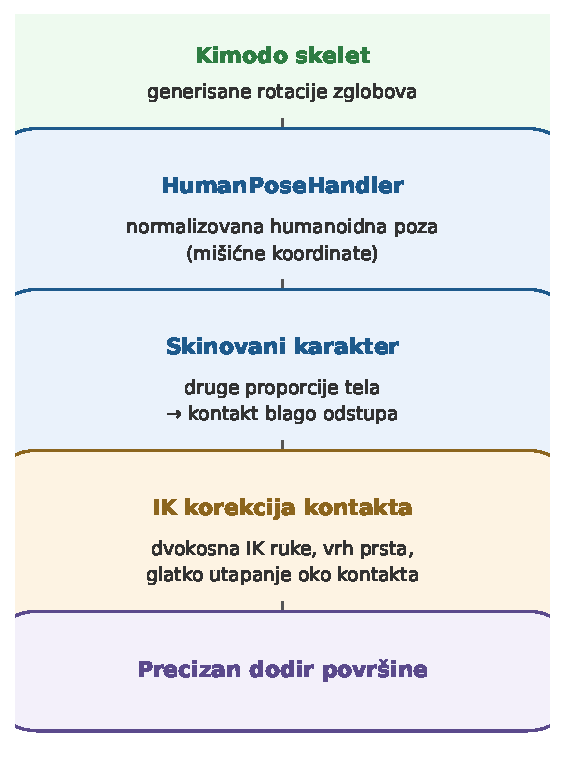
\includegraphics[width=0.5\textwidth]{figures/retarget.pdf}
    \caption{Prenos generisanog pokreta na skinovani karakter: rotacije se
    retargetuju kroz Mecanim humanoidnu reprezentaciju, a demonstrirani
    kontakti se zatim ponovo rešavaju inverznom kinematikom na ciljnom skeletu.}
    \label{fig:retarget_flow}
\end{figure}

Međutim, retargetovanje prvenstveno čuva relativnu konfiguraciju tela, a ne apsolutni položaj svakog efektora. Mala razlika u dužini nadlaktice ili podlaktice zato može dovesti do toga da šaka koja je na izvornom skeletu precizno dodirivala sto na ciljnom karakteru završi nekoliko centimetara iznad ili ispod površine.

Za slobodno kretanje takvo odstupanje često nije vidljivo, ali je za demonstrirane kontakte neprihvatljivo. Sistem zato čuva originalne pozicije i vremena kontaktnih ograničenja i nakon retargetovanja ponovo rešava položaj odgovarajuće ruke na ciljnom skeletu. Koristi se dvokosna inverzna kinematika sa vrhom prsta kao završnim efektorom.

Korekcija se ne uključuje naglo samo u jednom kadru. Njena težina se glatko povećava pri približavanju kontaktnom intervalu i zatim smanjuje nakon njega. Time se izbegava diskontinuitet između originalno generisanog pokreta i korigovanog položaja ruke.

Tokom implementacije identifikovan je i problem sa neutralnom pozom izvornog skeleta. Koren skeleta nalazi se u koordinatnom početku, dok stopala u neutralnoj konfiguraciji mogu imati negativnu visinu. Ukoliko se takva poza neposredno koristi za procenu razmere karaktera, dolazi do pogrešnog globalnog skaliranja i efekta lebdenja ili utapanja modela u pod. Pre inicijalnog vezivanja skelet se zato vertikalno pomera tako da najniža tačka stopala odgovara ravni poda.

Pored razmere, kalibriše se i globalno pomeranje karaktera. Odnos i smer translacije proveravaju se poređenjem putanje kukova izvornog i ciljnog skeleta. Time se lokalna artikulacija i globalno kretanje obrađuju odvojeno, što se pokazalo stabilnijim od direktnog kopiranja svih transformacija.

\subsection{Režija likova i prostorna ograđivanja pri reprodukciji}
\label{sec:direction}

Generisani lik nije statična animacija već objekat kojim korisnik može dalje da upravlja. Izborom lika (klikom na ekranu, odnosno usmeravanjem kontrolera i pritiskom na dugme u VR režimu) otvara se meni sa nekoliko mogućnosti.

\paragraph{Promena ponašanja.} Liku se može zadati novi tekstualni opis, izborom iz keširane liste ili slobodnim unosom, pri čemu se sva prostorna ograničenja originalne demonstracije zadržavaju. Ista prostorna konfiguracija tako se brzo ispituje sa različitim ponašanjima.

\paragraph{Vremenska osa i isecanje.} Uz meni se prikazuje vremenska osa klipa sa pokaznom glavom u realnom vremenu. Korisnik može da označi početak i kraj korisnog dela, nakon čega se reprodukuje samo izabrani isečak; isecanje je nedestruktivno i može se poništiti.

\paragraph{Nadovezivanje radnji.} Umesto zamene, sledeća radnja se može \emph{nadovezati}: sistem generiše novi klip usidren tačno na mestu gde se završava zadržani isečak tekućeg, i prelazi na njega kada pokazna glava dostigne tu granicu. Lik na taj način izvodi sekvencu radnji bez teleportovanja između njih.

\paragraph{Ručno pozicioniranje.} Izabrani lik se može pomeriti po podu i rotirati oko sopstvene ose (strelicama na tastaturi, odnosno palicama VR kontrolera), na primer da se izvedba blago odmakne od nameštaja, i po potrebi ukloniti iz scene.

\paragraph{Prostorna ograđivanja.} Pošto generativni model ne poznaje zidove ni nameštaj, reprodukcija primenjuje dva geometrijska ograničenja u svakom kadru: kukovi lika ne mogu napustiti pravougaonik prostorije (zadat eksplicitnim graničnim kolajderom ili procenjen iz registrovanih objekata), niti se naći duboko unutar otiska registrovanog komada nameštaja. Prekoračenje se koriguje pomeranjem celog lika kroz najbližu ivicu, pa lik na granici ,,hoda u mestu`` umesto da prođe kroz prepreku.

Kod ograde oko nameštaja pokazalo se da doslovno tvrdo sprovođenje ne valja: pri naginjanju preko ivice (što je legitiman deo posezanja) kukovi ritmično prelaze granicu otiska, pa korekcija koja se u svakom kadru primenjuje u punom iznosu proizvodi vidljivo ,,teleportovanje`` napred--nazad, naročito kod uglova gde smer izguravanja preskače između ivica. Konačna verzija zato dozvoljava plitko preklapanje (do $0.12\,m$), a korekciju primenjuje glatko, eksponencijalnim utapanjem ka ciljanoj vrednosti. Time se zadržava garancija da telo ne prolazi kroz nameštaj, dok naslanjanje i posezanje preko ivice ostaju vizuelno mirni. Ova ograđivanja važe za svaki reprodukovani klip, uključujući nadovezane radnje i generisanja bez prostornih ograničenja, i predstavljaju poslednju liniju odbrane geometrijske konzistentnosti scene.

% ============================================================
% 4. SCENARIO
% ============================================================

\section{Reprezentativni scenario}
\label{sec:scenario}

Kompletan tok sistema demonstriran je u laboratorijskoj virtuelnoj sceni sa radnim površinama, nameštajem i dva manipulatora Franka Emika Panda. Cilj scenarija nije simulacija konkretnog proizvodnog procesa, već prikaz kako se tekstualna semantika pokreta i prostorna demonstracija korisnika mogu kombinovati da bi se generisao čovek koji obavlja zadatak na tačno određenom mestu u sceni.

\begin{enumerate}
    \item Korisnik najpre bira ili unosi tekstualni opis ponašanja, na primer ,,osoba priđe stolu i pređe rukom po njegovoj površini``.

    \item U samoj sceni korisnik bira ciljnu površinu i pokazuje željeni prostorni deo zadatka. Može zadati samo tačku dodira, ali po potrebi može demonstrirati i putanju prilaska, čitav trag šake po površini ili jednu ili više ključnih poza.

    \item Unity iz geometrije scene proverava direktan prilaz i, ako je potrebno, generiše putanju koja zaobilazi prepreke. Sve demonstracije zatim se prevode u vremenski indeksirana Kimodo ograničenja.

    \item Server generiše pokret. Za već keširan tekstualni opis ovaj korak na korišćenoj konfiguraciji traje približno $10$--$15\,s$.

    \item Generisani karakter se pojavljuje na početku putanje, kreće se prema radnoj površini, zaobilazi prepreke, zaustavlja se na planiranom mestu i izvršava zadati kontakt.

    \item Korisnik zatim može izabrati već generisani karakter i dalje ga režirati: zadati mu novo ponašanje bez ponovnog zadavanja prostornih ograničenja, iseći koristan deo klipa na vremenskoj osi, nadovezati sledeću radnju koja počinje tamo gde se prethodna završila, ili ga ručno pomeriti i rotirati u sceni.
\end{enumerate}

Ovaj scenario objedinjuje sve glavne komponente sistema: interaktivno zadavanje ograničenja, planiranje u poznatoj sceni, generisanje pokreta modelom Kimodo, retargetovanje i korekciju kontakta. Ujedno ilustruje osnovnu namenu interfejsa, u kojoj korisnik ne animira čoveka direktno, već definiše uslove unutar kojih generativni model bira konkretnu realizaciju pokreta.

% \begin{figure}[H]
%     \centering
%     \begin{subfigure}[t]{0.48\textwidth}
%         \centering
%         \includegraphics[width=\linewidth]{figures/scene_demo.png}
%         \caption{Zadavanje ograničenja u sceni.}
%     \end{subfigure}
%     \hfill
%     \begin{subfigure}[t]{0.48\textwidth}
%         \centering
%         \includegraphics[width=\linewidth]{figures/scene_playback.png}
%         \caption{Generisani karakter izvodi zadatak.}
%     \end{subfigure}
%     \caption{Reprezentativni scenario u laboratorijskoj sceni.}
%     \label{fig:scenario}
% \end{figure}
% TODO: snimci ekrana (figures/scene_demo.png, figures/scene_playback.png)

% ============================================================
% 5. REZULTATI
% ============================================================

\section{Rezultati}
\label{sec:results}

Evaluacija trenutne implementacije usmerena je na funkcionalne osobine sistema koje su direktno relevantne za interaktivnu upotrebu: preciznost zadatih prostornih ograničenja, stabilnost reprodukcije u Unity-ju, uspešnost planiranja prilaza i vreme potrebno za generisanje.

\paragraph{Tačnost ograničenja.}
Poštovanje ograničenja provereno je direktnim merenjem na generisanom 77-zglobnom izlaznom skeletu. U testu sa istovremeno zadatim položajima leve i desne šake, nakon naknadne obrade rastojanje oba efektora od zadatih ciljeva u ključnom kadru iznosilo je $0.0$\,cm. Odstupanje položaja korena tela od zadatog horizontalnog položaja i visine bilo je manje od $1$\,cm.

Poređenja radi, ista demonstracija bez pravilnog razdvajanja ograničenja po rukama i bez vremenskog prozora oko ključne poze dovodila je do promašaja ciljeva reda $\approx38$\,cm. Rezultat pokazuje da preciznost ne potiče samo od osnovnog difuzionog generisanja, već od kombinacije uslovljavanja tokom uzorkovanja, odgovarajuće konstrukcije ograničenja i naknadnog \textit{constraint snapping} postupka.

Posebnim testovima leve i desne šake potvrđeno je i da transformacija između koordinatnih sistema Unity-ja i modela ne menja hiralnost skeleta.

\paragraph{Planiranje i ponašanje u sceni.}
Za testirane rasporede prepreka planer je pronalazio putanje koje izbegavaju pravougaone otiske nameštaja i dovode karakter do ciljnog mesta. Dodavanje ponovljenih krajnjih ograničenja uspešno sprečava nastavak hodanja nakon dostizanja radne površine. Izguravanje mesta stajanja iz otiska dodirnutog komada otklonilo je slučajeve u kojima je lik ulazio u duboki nameštaj, a tvrda ograđivanja pri reprodukciji (poglavlje~\ref{sec:direction}) garantuju da telo ni u nekontrolisanim delovima klipa ne napušta prostoriju niti prolazi kroz registrovane objekte. Sistem na taj način kompenzuje činjenicu da generativni model samostalno nema predstavu o semantici prepreke ili o tome da dostignuti cilj treba zadržati.

\paragraph{Retargetovanje i kontakt.}
Prenos preko Mecanim sistema omogućio je korišćenje skinovanog humanoidnog karaktera koji nema iste proporcije kao izvorni skelet. Lokalna IK korekcija vratila je demonstrirane kontakte na ciljnu površinu nakon retargetovanja. Korekcijom neutralne visine skeleta i kalibracijom globalne translacije uklonjeni su ranije primećeni artefakti lebdenja, utapanja u pod i pogrešne amplitude kretanja.

\paragraph{Performanse.}
Na računaru sa grafičkom karticom NVIDIA RTX 5070 Ti sa $12\,GB$ memorije, generisanje klipa od nekoliko sekundi sa 50 koraka uklanjanja šuma traje približno $10$--$15\,s$ kada je tekstualni opis prethodno kodiran. Takvo vreme nije dovoljno za kontrolu u realnom vremenu, ali omogućava interaktivni tok rada u kome korisnik zada demonstraciju, generiše ponašanje i zatim ga pregleda ili menja.

Kodiranje potpuno novog tekstualnog opisa predstavlja znatno skuplji korak. LLM2Vec enkoder sa približno 8 milijardi parametara u korišćenoj konfiguraciji izvršava se na procesoru i zahteva približno dva minuta. Međutim, dobijena reprezentacija se čuva u kešu, pa se ovo kašnjenje javlja samo pri prvoj upotrebi konkretnog opisa.

% ============================================================
% 6. DISKUSIJA
% ============================================================

\section{Diskusija: poteškoće metode i primenjene mere}
\label{sec:discussion}

Generisanje ponašanja difuzionim modelom pokreta pokazalo se upotrebljivim za interaktivnu scenu, ali gotovo nijedna ključna osobina sistema nije dobijena ,,besplatno``: većina je rezultat eksplicitnog usklađivanja između onoga što model nudi i onoga što konkretna scena zahteva. Tabela~\ref{tab:difficulties} sažima poteškoće uočene tokom razvoja i mere kojima su ublažene; detalji mehanizama dati su u poglavlju~\ref{sec:implementation}.

\begin{table}[H]
\centering
\small
\begin{tabular}{p{0.44\textwidth} p{0.5\textwidth}}
\toprule
\textbf{Poteškoća} & \textbf{Primenjena mera} \\
\midrule
Model nema svest o sceni: nameštaj, zidovi i roboti za njega ne postoje &
planiranje prilaza na klijentu (naduvani otisci, Liang--Barsky); izguravanje mesta stajanja iz otiska; ograda sobe i ublaženi \textit{keep-out} nameštaja pri reprodukciji \\
\addlinespace
Nema modela interakcije sa predmetima (hvatanje, nošenje, fizika objekata) &
kontakt sveden na precizno pozicijsko ograničenje šake uz \textit{constraint snapping} i IK korekciju; prava manipulacija predmetima ostavljena za fizičku simulaciju (budući rad) \\
\addlinespace
Ograničenja važe samo u svojim kadrovima: u ,,praznim`` delovima klipa lik prehodava cilj ili odluta &
ponovljena krajnja ograničenja do kraja klipa; prozori držanja poza; vremensko zgušnjavanje traga dodira \\
\addlinespace
Redak pin (jedan kadar) je preslab signal difuzionom vođenju &
držanje svake poze u kratkom neprekidnom prozoru; pojačano vođenje ograničenja; skupovi imenovani po ruci (uslov naknadne obrade) \\
\addlinespace
Protivrečna ili neizvodljiva ograničenja destabilizuju uzorkovanje, do potpuno degenerisanog pokreta &
provere izvodljivosti pri snimanju (sfera dohvata, minimalno vreme putovanja, verodostojne visine vizira); adaptivna visina kukova za niske ciljeve \\
\addlinespace
Povremeno ,,čudno`` ponašanje: semantika prompta boji sve neograničene delove klipa &
kurirani osnovni promptovi; podela opisa na uzastopne segmente; režija --- zamena ponašanja, isecanje lošeg dela, nadovezivanje, ručno pozicioniranje \\
\addlinespace
Retargetovanje čuva uglove zglobova, ne apsolutne pozicije kontakata &
IK korekcija kontakta na ciljnom skeletu; kalibracija razmere i globalne translacije; ispravka neutralne poze \\
\addlinespace
Latencija: $\sim$2\,min kodiranja novog opisa, $10$--$15\,s$ generisanja &
keširanje tekstualnih reprezentacija (lenji enkoder); tok rada demonstracija $\to$ generisanje $\to$ pregled i režija umesto upravljanja u realnom vremenu \\
\bottomrule
\end{tabular}
\caption{Poteškoće generisanja difuzionim modelom u interaktivnoj VR sceni i mere kojima su usklađene.}
\label{tab:difficulties}
\end{table}

% ============================================================
% 7. OGRANIČENJA I BUDUĆI RAD
% ============================================================

\section{Ograničenja i budući rad}
\label{sec:limitations}

\paragraph{Ograničena svest o geometriji scene.}
Generativni model ne dobija geometriju virtuelnog okruženja. Trenutna implementacija ovaj problem delimično rešava tako što na strani klijenta planira putanju korena tela. Time se izbegavaju prepreke tokom globalnog kretanja, ali nije garantovano da pojedinačni delovi tela tokom slobodno generisanih gestova neće preseći objekte u sceni. Prirodno proširenje sistema bilo bi automatsko detektovanje takvih kolizija i ponovno generisanje ili lokalna korekcija problematičnih segmenata.

\paragraph{Parcijalno posmatranje korisnika.}
Postojeća VR oprema direktno meri samo vizir i dva kontrolera. Položaji laktova, kolena i ostalih segmenata tela zato nisu deo demonstracije. Sistem namerno ostavlja te stepene slobode generativnom modelu, što omogućava prirodnu varijabilnost, ali istovremeno znači da korisnik ne može precizno da demonstrira kompletnu konfiguraciju tela. Dodatni trackeri ili procena poze iz spoljne kamere omogućili bi bogatije ograničavanje.

\paragraph{Orijentacija šake i manipulacija objektima.}
Trenutni sistem prvenstveno koristi položaj šake kao kontaktno ograničenje. Za zadatke u kojima je važna precizna orijentacija šake ili hvatanje objekta bilo bi potrebno uključiti dodatne rotacione uslove i model interakcije sa objektom.

\paragraph{Fizička izvodljivost.}
Kimodo generiše kinematičke sekvence. Model ne izračunava sile, momente zglobova niti kontaktne reakcije, pa sama generisana sekvenca nije garancija da isti pokret može dinamički da izvede fizički simulirano ili stvarno telo. Jedan od planiranih nastavaka rada jeste korišćenje sačuvanih demonstracionih konfiguracija kao ulaza u fizičku simulaciju, gde bi se generisani pokret mogao dodatno proveravati i prilagođavati.

\paragraph{Dužina i glatkoća sekvence.}
Trenutni tok rada zasnovan je na generisanju relativno kratkih klipova, a duži zadaci se grade nadovezivanjem (poglavlje~\ref{sec:direction}). Nadovezani klip je usidren na \emph{mestu} završetka prethodnog, ali se konfiguracija tela u trenutku prelaza ne prenosi, pa je prelaz trenutna zamena poze umesto glatkog stapanja. Prirodno proširenje bilo bi prosleđivanje završne poze kao početnog ograničenja sledećeg klipa ili kratko vremensko stapanje na granici.

\paragraph{Interfejs.}
Veći deo ranije planiranih poboljšanja interfejsa u međuvremenu je realizovan (štap-figure snimljenih poza, vremenska osa sa isecanjem, vizuelno razlikovanje tipova ograničenja bojama markera). Otvorena poboljšanja uključuju ponovno korišćenje isečenih segmenata kao gradivnih blokova, bogatiji VR meni ravnopravan onom na ekranu, i eksplicitno definisane zone u kojima je kretanje odnosno interakcija dozvoljena.

% ============================================================
% 7. ZAKLJUČAK
% ============================================================

\section{Zaključak}
\label{sec:conclusion}

U ovom radu razvijen je interaktivni sistem za generisanje ljudskog pokreta u virtuelnoj stvarnosti koji kombinuje semantičke instrukcije zadate tekstom i prostorna ograničenja zadata direktnom demonstracijom korisnika. Umesto da korisnik ručno animira virtuelnog čoveka ili numerički unosi koordinate, željeni prostorni deo ponašanja može da pokaže hodanjem, pomeranjem kontrolera po površini ili zauzimanjem ključne poze.

Glavni tehnički problem nije samo generisanje pokreta modelom Kimodo, već prevođenje između tri različite reprezentacije istog zadatka: korisničke demonstracije u VR prostoru, kinematičkih ograničenja generativnog modela i konačne animacije humanoidnog karaktera u Unity sceni. U okviru sistema zato su razvijeni postupci za konstrukciju ograničenja iz parcijalno praćene poze, planiranje putanje kroz poznatu scenu, transformaciju između koordinatnih sistema, retargetovanje i lokalnu korekciju kontakta.

Rezultati pokazuju da retka demonstracija može biti dovoljna da se generativni model prostorno usmeri bez potpunog određivanja pokreta. Eksplicitno zadate pozicije šaka nakon naknadne obrade dostižu ciljeve praktično bez merljivog odstupanja na izvornom skeletu, dok dodatna IK korekcija omogućava očuvanje kontakta i nakon prenosa na karakter drugačijih proporcija.

Takav pristup posebno je interesantan za virtuelna okruženja namenjena saradnji čoveka i robota. Korisnik može brzo da formira različita ljudska ponašanja u konkretnoj robotskoj sceni bez potrebe da svako od njih unapred snimi ili ručno animira. Difuzioni model određuje prirodnu realizaciju pokreta, dok VR demonstracija određuje delove ponašanja koji moraju biti prostorno precizni.

Dalji razvoj može da poveže ovakav interaktivni generator sa fizičkom simulacijom i robotskim planerima. Time bi ista demonstracija mogla da posluži prvo za generisanje različitih mogućih ljudskih pokreta, a zatim za analizu njihove fizičke izvodljivosti i uticaja na robota koji sa čovekom deli radni prostor.

\bibliographystyle{plain}
\bibliography{references}

\end{document}
